We implemented the lexicographic order algorithm ($\LT$, Eq.~\ref{eq:general_lex_order}) using the BGV scheme~\cite{BGV12}.
The code is written in the HElib library~\cite{HElib}.
For a fair comparison with the prior work, we also implemented the algorithm of Tan et al.~\cite{TLWRK20}.
The code will be publicly available.
In all the experiments, we used an average commodity laptop equipped with an Intel Dual-Core i5-7267U CPU (running at 3.1 GHz) and 8 GB of RAM.
Multi-threading was turned off.

In the results presented below, the following notation is used:
\begin{description}
  \item[$p:$] the plaintext modulus of the BGV scheme;
  \item[$q:$] the initial ciphertext modulus of the BGV scheme;
  \item[$m:$] the cyclotomic order of the ring $\intring$;
  \item[$n:$] the degree of the ring $\intring$ ($n = \phi(m)$);
  \item[$\ell:$] the number of SIMD slots;
  \item[$d:$] the dimension of a slot subspace used for digit encoding ($d'$ in Eq.~\ref{eq:general_lex_order});
  \item[$l:$] the dimension of digit vectors encoding input integers over $\F_p^d$;
  \item[$k:$] the number of input integers encoded in one ciphertext ($k = \floor{\ell/l}$).
\end{description}

In all the experiments, the encryption parameters of BGV are chosen according to the following strategy.
The plaintext modulus $p$ is a prime number such that SIMD slots are isomorphic to a finite field.
Next, we choose the order $m$ of $\intring$ with large enough $n$ to support our homomorphic algorithms ($n > 12000$).
The order of $p$ modulo $m$ should be as small as possible, which maximizes the number of SIMD slots, thus reducing the amortized running time of our algorithms.
In addition, $m$ is chosen to be a prime number or a product of a few primes.
This constraint makes sure that the slot permutation group is cyclic or a product of a few cyclic groups, which results in a better performance (for more details, see \cite[Appendix C.3]{GHS12}).

Every input integer is encoded into exactly one ciphertext.
First, it is decomposed into a vector of $l$ digits over $\F_p^d$ (see Section~\ref{sec:comparison_of_large_integers}).
Then each digit embedded into one SIMD slot.
Thus, each ciphertext encrypts exactly $k = \ell/l$ integers.

To compare our algorithms with the state of the art, we ran the lexicographic order algorithm ($\LT$) to compute the less-than function on 64-bit integers.
The results of these experiments are presented in Table~\ref{table:comparison_circuit_results}.
In addition, we ran the direct sorting and the array minimum algorithms from Section~\ref{sec:applications}; see Tables~\ref{table:sorting_circuit_results} and~\ref{table:minimum_circuit_results}, respectively.

We ran our algorithms with $p \in [3,659]$.
However, Table~\ref{table:comparison_circuit_results} contains the results with the best observed amortized running time and the best results for small $p$'s, where the bivariate and the univariate comparison circuits have a comparable running time.
For the sorting and the array minimum applications (Tables~\ref{table:sorting_circuit_results} and~\ref{table:minimum_circuit_results}), we showed only the results with $p$ and $m$ supporting reasonable security levels and giving the best running time for arrays of length $N=64$.

\begin{table*}[h]
  \centering
  \begin{tabular*}{.9\textwidth}{@{\extracolsep{\fill} } p{3.0cm} p{0.5cm} p{1.0cm} p{1.0cm} p{1.0cm} p{1.0cm} p{2.0cm} p{2.0cm}}
    \toprule
    $(p,m,n)$ & Type & $(d,l)$   &  $\log_2 q$ & $\lambda$    & $k$ & Total time, s & Amortized time per slot, ms \\
    \cmidrule(lr){1-1}\cmidrule(lr){2-8}
    %$(3,34511,34510)$  & \cite{TLWRK20}  & $(1,41)$  & $>320$ & $49$   & 7.10   & 145 \\
    %$(3,34511,34510)$  & \cite{TLWRK20}  & $(2,21)$  & $>320$ & $96$   & 14.80  & 154 \\
    %$(3,34511,34510)$  & \cite{TLWRK20}  & $(4,11)$  & $>320$ & $184$  & 20.60  & 112 \\
    %$(3,34511,34510)$  & \cite{TLWRK20}  & $(5,9)$   & $>320$ & $225$  & 23.67  & 105 \\
    \multirow{3}{*}{$(3,34511,34510)$}  & \cite{TLWRK20}  & $(6,7)$   & $324$ & $298$ & $290$  & 26.24  & 90 \\
    %$(3,34511,34510)$  & \cite{TLWRK20}  & $(11,4)$  & $>380$ & $507$  & 48.25  & 95 \\
    %$(3,34511,34510)$  & B               & $(1,41)$  & $>320$ & $49$   & 6.36   & 130 \\
    %$(3,34511,34510)$  & B               & $(2,21)$  & $>310$ & $96$   & 12.33  & 128 \\
    %$(3,34511,34510)$  & B               & $(4,11)$  & $>310$ & $184$  & 16.69  & 91 \\
    %$(3,34511,34510)$  & B               & $(5,9)$   & $>320$ & $225$  & 18.57  & 83 \\
    %$(3,34511,34510)$  & B               & $(6,7)$   & $>310$ & $290$  & 20.51  & 71 \\
      & B               & $(6,7)$   & $324$ & $298$ & $290$  & 20.17  & 70 \\
    %$(3,34511,34510)$  & B               & $(11,4)$  & $385$ & $226$ & $507$  & 35.45  & 70 \\
    %$(3,34511,34510)$  & U               & $(1,64)$  & $>320$ & $31$   & 5.18   & 167 \\
    %$(3,34511,34510)$  & U               & $(2,32)$  & $>310$ & $63$   & 7.84   & 124 \\
    %$(3,34511,34510)$  & U               & $(4,16)$  & $>310$ & $126$  & 10.11  & 80 \\
    %$(3,34511,34510)$  & U               & $(8,8)$   & $>360$ & $253$  & 16.43  & 65 \\
      & U               & $(16,4)$  & $472$ & $189$ & $507$  & 28.45  & 56 \\
    \cmidrule(lr){1-1}\cmidrule(lr){2-8}
    %$(5,19531,19530)$  & \cite{TLWRK20}  & $(1,28)$  & $>290$ & $99$   & 4.68   & 47 \\
    %$(5,19531,19530)$  & \cite{TLWRK20}  & $(4,7)$   & $>295$ & $398$  & 14.33  & 36 \\
    \multirow{3}{*}{$(5,19531,19530)$}  & \cite{TLWRK20}  & $(7,4)$   & $324$ & $155$ & $697$  & 24.97  & 36 \\
    %$(5,19531,19530)$  & B               & $(1,28)$  & $>290$ & $99$   & 3.09   & 31 \\
    %$(5,19531,19530)$  & B               & $(2,14)$  & $>290$ & $199$  & 5.72   & 29 \\
    %$(5,19531,19530)$  & B               & $(4,7)$   & $>295$ & $398$  & 8.98   & 23 \\
      & B               & $(7,4)$   & $324$ & $155$ & $697$  & 14.50  & 21 \\
    %$(5,19531,19530)$  & U               & $(1,41)$  & $>330$ & $68$   & 3.04   & 45 \\
    %$(5,19531,19530)$  & U               & $(2,21)$  & $>330$ & $132$  & 4.38   & 33 \\
    %$(5,19531,19530)$  & U               & $(3,14)$  & $>320$ & $199$  & 5.17   & 26 \\
    %$(5,19531,19530)$  & U               & $(4,11)$  & $>320$ & $253$  & 6.11   & 24 \\
    %$(5,19531,19530)$  & U               & $(6,7)$   & $>340$ & $398$  & 8.71   & 22 \\
      & U               & $(7,6)$   & $354$ & $141$ & $465$  & 9.89  & 21 \\
    \cmidrule(lr){1-1}\cmidrule(lr){2-8}
    %$(7,14009,14008)$  & U               & $(1,32)$  & $>330$ & $25$   & 1.88   & 75 \\
    %$(7,14009,14008)$  & U               & $(2,16)$  & $>330$ & $51$   & 3.69   & 72 \\
    %$(7,14009,14008)$  & U               & $(4,8)$   & $>310$ & $103$  & 5.21   & 51 \\
    %$(7,14009,14008)$  & U               & $(8,4)$   & $342$ & $102$ & $206$  & 9.11   & 44 \\
    %$(7,14009,14008)$  & B               & $(1,23)$  & $>330$ & $35$   & 1.88   & 54 \\
    %$(7,14009,14008)$  & B               & $(2,12)$  & $>330$ & $68$   & 3.67   & 54 \\
    %$(7,14009,14008)$  & B               & $(4,6)$   & $>320$ & $137$  & 5.34   & 39 \\
    %$(7,14009,14008)$  & B               & $(6,4)$   & $>310$ & $206$  & 6.91   & 34 \\
    %$(7,14009,14008)$  & B               & $(8,3)$   & $354$  & ?  & $274$ & ?19.30   & ?71 \\
    %$(7,14009,14008)$  & \cite{TLWRK20}  & $(6,4)$   & $324$  & $206$  & ? & ?26.24   & ?128 \\
    %$(7,14009,14008)$  & \cite{TLWRK20}  & $(8,3)$   & $354$  & ?  & $274$ & ?32.30   & ?118 \\
    %$(7,14009,14008)$  & \cite{TLWRK20}  & $(12,2)$  & $384$  & $412$  & ? & ?50.93   & ?124 \\
    \multirow{3}{*}{$(7,20197,19116)$}  & \cite{TLWRK20}  & $(6,4)$   & $354$ & $137$ & $531$  & 37.50  & 71 \\
    %$(7,20197,19116)$  & B               & $(1,23)$  & $>350$ & $92$   & 6.55   & 71 \\
    %$(7,20197,19116)$  & B               & $(2,12)$  & $>320$ & $177$  & 10.11  & 57 \\
    %$(7,20197,19116)$  & B               & $(3,8)$   & $>320$ & $265$  & 12.33  & 47 \\
    %$(7,20197,19116)$  & B               & $(4,6)$   & $>320$ & $354$  & 15.37  & 43 \\
      & B               & $(6,4)$   & $354$ & $137$ & $531$  & 21.35  & 40 \\
    %$(7,20197,19116)$  & B               & $(8,3)$   & $>380$ & $708$  & 29.67  & 42 \\
    %$(7,20197,19116)$  & U               & $(1,32)$  & $>350$ & $66$   & 5.22   & 79 \\
    %$(7,20197,19116)$  & U               & $(2,16)$  & $>350$ & $132$  & 6.81   & 52 \\
    %$(7,20197,19116)$  & U               & $(4,8)$   & $>350$ & $265$  & 9.27   & 35 \\
      & U               & $(8,4)$   & $406$ & $110$ & $531$  & 16.53  & 31 \\

    \cmidrule(lr){1-1}\cmidrule(lr){2-8}
    %$(11,15797,15796)$ & \cite{TLWRK20}  & $(1,19)$   & $360$  & ? & $75$  & 8.25  & 110 \\
    %$(11,15797,15796)$ & \cite{TLWRK20}  & $(2,10)$   & $360$  & ? & $143$ & 16.96 & 119 \\
    %$(11,15797,15796)$ & \cite{TLWRK20}  & $(4,5)$    & $360$  & ? & $287$ & 29.29 & 103 \\
    \multirow{3}{*}{$(11,15797,15796)$} & \cite{TLWRK20}  & $(5,4)$    & $342$  & $162$ & $359$ & 35.20 & 99 \\
    %$(11,15797,15796)$ & \cite{TLWRK20}  & $(10,2)$   & $378$  & ? & $718$ & 76.39 & 107 \\

     & B               & $(5,4)$    & $342$  & $162$ & $359$ & 22.76 & 64 \\

    %$(11,15797,15796)$ & U               & $(1,25)$  & $378$ & ?     & $57$   & ?2.94   & ?52 \\
    %$(11,15797,15796)$ & U               & $(2,13)$  & $354$ & ?     & $110$  & ?4.62   & ?42 \\
    %$(11,15797,15796)$ & U               & $(3,9)$   & $378$ & ?     & $159$  & ?6.72   & ?43 \\
    %$(11,15797,15796)$ & U               & $(4,7)$   & $354$ & ?     & $205$  & ?7.62   & ?38 \\
     & U               & $(5,5)$   & $378$ & $145$     & $287$  & 9.79   & 35 \\
    %$(11,15797,15796)$ & U               & $(7,4)$   & $385$ & ?     & $359$  & ?12.72  & ?36 \\
    %$(11,15797,15796)$ & U               & $(9,3)$   & $>410$ & $478$  & ?  & ? \\

    \cmidrule(lr){1-1}\cmidrule(lr){2-8}
    %$(11,21963,14640)$ & U               & $(1,25)$  & $>360$ & $73$   & 4.59   & 63 \\
    %$(11,21963,14640)$ & U               & $(2,13)$  & $>360$ & $140$  & 6.64   & 47 \\
    %$(11,21963,14640)$ & U               & $(3,9)$   & $>360$ & $203$  & 8.70   & 43 \\
    %$(11,21963,14640)$ & U               & $(4,7)$   & $>350$ & $261$  & 9.67   & 37 \\
    %$(11,21963,14640)$ & U               & $(5,5)$   & $>360$ & $366$  & 12.43  & 34 \\

    %$(11,21963,14640)$ & \cite{TLWRK20}  & $(5,4)$    & $354$  & ? & $457$ & 47.84 & 105 \\

    %$(13,30941,30940)$ & \cite{TLWRK20}   & $(4,5)$   & $378$   & ? & $1237$ & 73.22 & 60 \\
    \multirow{3}{*}{$(13,30941,30940)$} & \cite{TLWRK20}   & $(5,4)$   & $354$   & $338$ & $1547$ & 82.02 & 54 \\

     & B                & $(5,4)$   & $354$   & $338$ & $1547$ & 54.05 & 35 \\

    %$(13,30941,30940)$ & U                & $(1,23)$  & $378$   & ? & $269$  & ?6.17  & ?23 \\
    %$(13,30941,30940)$ & U                & $(2,12)$  & $378$   & ? & $515$  & ?9.80  & ?20 \\
     & U                & $(4,6)$   & $378$   & $313$ & $1031$ & 15.56 & 16 \\
    %$(13,30941,30940)$ & U                & $(5,5)$   & $385$   & ? & $1237$ & ?18.96 & ?16 \\

    \cmidrule(lr){1-1}\cmidrule(lr){2-8}
    %$(17,41761,41760)$ & \cite{TLWRK20}   & $(1,16)$   & $486$   & ? & $326$  & ?39.95 & ?123 \\
    %$(17,41761,41760)$ & \cite{TLWRK20}   & $(2,8)$    & $456$   & ? & $652$  & ?73.75  & ?114 \\
    \multirow{3}{*}{$(17,41761,41760)$} & \cite{TLWRK20}   & $(4,4)$    & $413$   & $402$ & $1305$ & 130.81 & 101 \\
    %$(17,41761,41760)$ & \cite{TLWRK20}   & $(8,2)$    & $432$   & ? & $2610$ & ?276.25 & ?106 \\

     & B                & $(4,4)$    & $413$   & $402$ & $1305$ & 91.14  & 70 \\

    %$(17,41761,41760)$ & U                & $(2,11)$   & $521$   & ? & $474$ & ?21.70 & ?46 \\
    %$(17,41761,41760)$ & U                & $(3,7)$    & $472$   & ? & $745$  & ?23.55 & ?32 \\
    %$(17,41761,41760)$ & U                & $(6,4)$    & $472$   & ? & $1305$ & ?39.96 & ?31 \\
     & U                & $(7,3)$    & $472$   & $344$ & $1740$ & 45.29 & 27 \\

    \cmidrule(lr){1-1}\cmidrule(lr){2-8}
    %$(19,29989,29988)$ & \cite{TLWRK20}   & $(1,16)$   & $373$   & ? & $208$  & ?25.96  & ?125 \\
    %$(19,29989,29988)$ & \cite{TLWRK20}   & $(2,8)$    & $373$   & ? & $416$  & ?55.49  & ?134 \\
    \multirow{3}{*}{$(19,29989,29988)$} & \cite{TLWRK20}   & $(4,4)$    & $378$   & $302$ & $833$  & 101.75 & 123 \\
    %$(19,29989,29988)$ & \cite{TLWRK20}   & $(8,2)$    & $413$   & ? & $1666$  & ?205.44 & ?124 \\

    & B                 & $(4,4)$    & $378$   & $302$ & $833$  & 69.92 & 84 \\

    & U                 & $(5,4)$    & $385$   & $296$ & $833$  & 20.76 & 25 \\
    %& U                 & $(7,3)$    & $440$   & ? & $1110$  & ?32.44 & ?30 \\

    \cmidrule(lr){1-1}\cmidrule(lr){2-8}
    %\multirow{3}{*}{$(23,37745,30192)$} & \cite{TLWRK20}   & $(1,15)$    & $385$   & ? & $167$  & ?38.61 & ?232 \\
    %\multirow{3}{*}{$(23,37745,30192)$} & \cite{TLWRK20}   & $(2,8)$     & $385$   & ? & $314$  & ?82.38 & ?263 \\
    %\multirow{3}{*}{$(23,37745,30192)$} & \cite{TLWRK20}   & $(3,5)$     & $385$   & ? & $503$  & ?120.37 & ?240 \\
    \multirow{3}{*}{$(23,37745,30192)$} & \cite{TLWRK20}   & $(5,3)$     & $413$   & $275$ & $838$  & 194.41 & 232 \\
    %\multirow{3}{*}{$(23,37745,30192)$} & \cite{TLWRK20}   & $(8,2)$     & $431$   & ? & $1258$  & ?329.64 & ?263 \\

    & B                 & $(5,3)$    & $413$   & $275$ & $838$  & 135.40 & 162 \\

    %& U                 & $(3,6)$    & $431$   & ? & $419$  & ?25.77 & ?62 \\
    %& U                 & $(5,4)$    & $431$   & ? & $629$  & ?37.90 & ?61 \\
    %& U                 & $(6,3)$    & $431$   & ? & $838$   & ?39.26 & ?47 \\
    & U                 & $(9,2)$    & $456$   & $245$ & $1258$  & 56.49 & 45 \\

    \cmidrule(lr){1-1}\cmidrule(lr){2-8}
    %\multirow{3}{*}{$(29,18157,17820)$} & \cite{TLWRK20}   & $(1,14)$    & $378$   & ? & $212$  & ?25.96 & ?123 \\
    %\multirow{3}{*}{$(29,18157,17820)$} & \cite{TLWRK20}   & $(2,7)$    & $378$   & ? & $424$  & ?50.09 & ?119 \\
    %\multirow{3}{*}{$(29,18157,17820)$} & \cite{TLWRK20}   & $(3,5)$    & $378$   & ? & $594$  & ?74.92 & ?127 \\
    %\multirow{3}{*}{$(29,18157,17820)$} & \cite{TLWRK20}   & $(4,4)$    & $378$   & ? & $742$  & ?98.71 & ?134 \\
    \multirow{3}{*}{$(29,18157,17820)$} & \cite{TLWRK20}   & $(5,3)$    & $360$   & $175$ & $990$  & 103.28 & 105 \\

    & B                 & $(5,3)$    & $360$   & $175$ & $990$  & 70.82 & 72 \\

    %& U                 & $(5,4)$    & $413$   & ? & $742$   & ?23.28 & ?24 \\
    & U                 & $(6,3)$    & $413$   & $150$ & $990$   & 19.98 & 21 \\

    \cmidrule(lr){1-1}\cmidrule(lr){2-8}
    %\multirow{3}{*}{$(31,52053,34700)$} & \cite{TLWRK20}   & $(1,13)$    & $559$   & ? & $533$  & ?104.26 & ?196 \\
    %\multirow{3}{*}{$(31,52053,34700)$} & \cite{TLWRK20}   & $(2,7)$     & $522$   & ? & $991$  & ?179.53 & ?182 \\
    %\multirow{3}{*}{$(31,52053,34700)$} & \cite{TLWRK20}   & $(3,5)$     & $522$   & ? & $1388$  & ?271.72 & ?196 \\
    \multirow{3}{*}{$(31,52053,34700)$} & \cite{TLWRK20}   & $(5,3)$     & $512$   & $252$ & $2313$  & 437.11 & 189 \\

    & B                 & $(5,3)$     & $512$   & $252$ & $2313$  & 293.27 & 127 \\

    & U                 & $(4,4)$     & $512$   & $252$ & $1735$  & 46.58 & 27 \\      
    \bottomrule
  \end{tabular*}
  \caption{\textbf{Less-than function via different methods.} The running time of our lexicographic order algorithms and the algorithm of Tan et al.~\cite{TLWRK20} to compare 64-bit integers with encryption parameters supporting $\lambda$ bits of security. The second column (Type) indicates which comparison circuit is used: the univariate (U), bivariate from this work (B) or bivariate one from~\cite{TLWRK20}. The total time is averaged over 50 trials.}
  \label{table:comparison_circuit_results}
\end{table*}

\begin{table*}[h]
  \centering
  \begin{tabular*}{.9\textwidth}{@{\extracolsep{\fill} } p{3.0cm} p{1.0cm} p{1.0cm} p{1.0cm} p{1.0cm} p{2.0cm} p{2.0cm}}
    \toprule
    $(p,m,n)$ & $(d,l)$   &  $\log_2 q$ & $\lambda$    & $k$ & Total time, s & Amortized time per slot, ms \\
    \cmidrule(lr){1-1}\cmidrule(lr){2-7}
    %$(67,26881,26880)$ & U               & $(1,13)$  & $>460$ & $413$  & 8.21   & 20 \\
    %$(67,26881,26880)$ & U               & $(2,7)$   & $>460$ & $768$  & 14.57  & 19 \\
    %$(67,26881,26880)$ & U               & $(4,4)$   & $>460$ & $1344$ & 26.63  & 20 \\
    %$(67,26881,26880)$ & U               & $(5,3)$   & $>480$ & $1792$ & 35.37  & 19 \\

    %$(109,24061,24060)$ & U              & $(1,12)$  & $>480$ & $401$  & 8.99   & 22 \\
    %$(109,24061,24060)$ & U              & $(2,6)$   & $>460$ & $802$  & 16.11  & 20 \\
    %$(109,24061,24060)$ & U              & $(3,4)$   & $>440$ & $1203$ & 21.22  & 18 \\
    %$(109,24061,24060)$ & U              & $(4,3)$   & $>440$ & $1604$ & 29.89  & 19 \\

    %$(131,17293,17292)$ & U              & $(1,11)$  & $>465$ & $524$  & 6.57   & 13 \\
    %$(131,17293,17292)$ & U              & $(2,6)$   & $>465$ & $960$  & 11.81  & 12 \\
    $(131,17293,17292)$               & $(3,4)$   & $431$ & $96$ & $1441$ & 16.07  & 11 \\

    %$(167,28057,28056)$ & U              & $(1,11)$  & $>520$ & $850$  & 12.38  & 15 \\
    %$(167,28057,28056)$ & U              & $(2,6)$   & $>520$ & $1558$ & 22.36  & 14 \\
    $(167,28057,28056)$              & $(3,4)$   & $494$ & $146$ & $2338$ & 30.69  & 13 \\

    %$(173,30103,30102)$ & U              & $(1,10)$  & $>520$ & $1003$ & 13.36  & 13 \\
    $(173,30103,30102)$               & $(2,5)$   & $521$ & $148$ & $2006$ & 24.57  & 12 \\
    %$(173,30103,30102)$ & U              & $(3,4)$   & $>490$ & $2508$ & 32.60  & 13 \\

    %$(401,23029,23028)$ & U              & $(1,9)$   & $>570$ & $852$  & 14.50  & 17 \\
    %$(401,23029,23028)$ & U              & $(3,3)$   & $>540$ & $2558$ & 35.15  & 14 \\
    \bottomrule
  \end{tabular*}
  \caption{\textbf{Less-than function via the univariate circuit.} The best empirical running time of our lexicographic order algorithm to compare 64-bit integers with encryption parameters supporting $\lambda$ bits of security. The algorithm is based on the univariate circuit. The total time is averaged over 50 trials.}
  \label{table:univariate_circuit_results}
\end{table*}

\begin{figure}
    \centering
    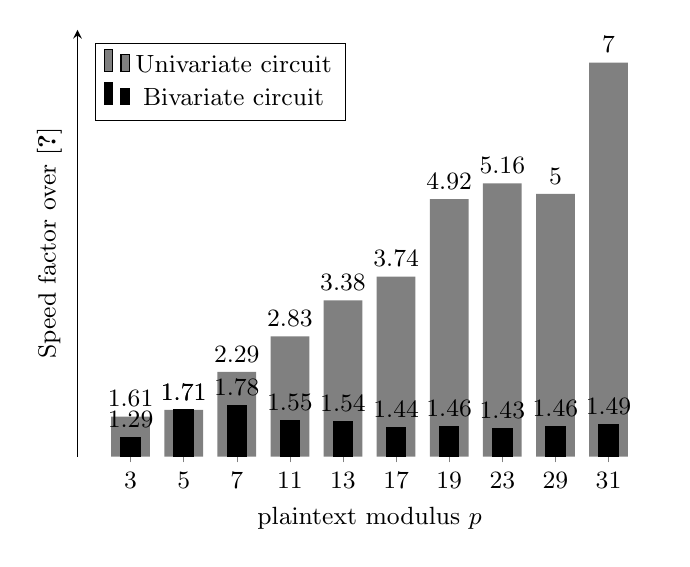
\begin{tikzpicture}
        \begin{axis}[
            width=9.0cm, 
            height=7cm, 
            %ymin=0, ymax=240,
            ymin=1, ymax=7.5, 
            xmin=0, xmax=11, 
            axis y line = left, axis x line = bottom,
            x axis line style = {draw=none},
            xtick = {1,2,3,4,5,6,7,8,9,10},
            xticklabels = {3,5,7,11,13,17,19,23,29,31},
            ylabel = {Speed factor over \cite{TLWRK20}},
            xlabel = {plaintext modulus $p$},
            ytick = \empty,
            legend pos = north west,
            font = \small
            ]
                %\addplot[ybar, ybar legend, fill=white, bar width = 15pt, nodes near coords] coordinates {(1, 90) (2, 36) (3,71) (4,99) (5,54) (6,101) (7,123) (8,232) (9,105) (10,189)};
                %\addlegendentry{\cite{TLWRK20}}
                %\addplot[ybar, ybar legend, fill=gray, bar width = 10pt, nodes near coords] coordinates {(1, 70) (2, 21) (3,40) (4,64) (5,35) (6,70) (7,84) (8,162) (9,72) (10,127)};
                %\addlegendentry{Bivariate circuit}
                %\addplot[ybar, ybar legend, fill=black, bar width = 5pt, nodes near coords] coordinates {(1, 56) (2, 21) (3,31) (4,35) (5,16) (6,27) (7,25) (8,45) (9,22) (10,27)};
                %\addlegendentry{Univariate circuit}
                \addplot[ybar, ybar legend, fill=gray, draw=none, bar width = 14pt, nodes near coords] coordinates {(1, 1.61) (2, 1.71) (3,2.29) (4,2.83) (5,3.38) (6,3.74) (7,4.92) (8,5.16) (9,5) (10,7)};
                \addlegendentry{Univariate circuit}
                \addplot[ybar, ybar legend, fill=black, bar width = 7pt, nodes near coords] coordinates {(1, 1.29) (2, 1.71) (3,1.78) (4,1.55) (5,1.54) (6,1.44) (7,1.46) (8,1.43) (9,1.46) (10,1.49)};
                \addlegendentry{Bivariate circuit}
                
            \end{axis}
    \end{tikzpicture}
    \caption{\textbf{Less-than function via different methods.} The running time speedup factor of our lexicographic order algorithms over the algorithm of Tan et al.~\cite{TLWRK20}. These factors are computed using the data from Table~\ref{table:comparison_circuit_results}.}
    \label{fig:comparison_circuit_results}
\end{figure}

As shown in Table~\ref{table:comparison_circuit_results} and Figure~\ref{fig:comparison_circuit_results}, our lexicographic order circuits have a better running time than the prior work of Tan et al.~\cite{TLWRK20} even for small plaintext moduli.
In particular, using our bivariate circuit, the less-than function is 1.71 times faster than with the circuit of Tan et al. on their fastest set of parameters ($(p,d,l) = (5,7,4)$).
The best running time per integer was achieved by our univariate circuit, which outperforms any bivariate circuit for any $p > 5$ at the cost of larger encryption parameters.
Table~\ref{table:univariate_circuit_results} shows that for $p=131$, the univariate circuit takes only 11 milliseconds to compare two 64-bit integers, which is more than 3 times faster than the best running time achieved by the circuit of Tan et al.

\begin{table}[h]
  \centering
  \begin{tabular*}{.45\textwidth}{ p{0.3cm} p{0.7cm} p{0.8cm} p{1cm} p{1.3cm} p{1.5cm}}
    \toprule
    $N$     & $\log_2 q$    & \#Trials  & Average total time, s & Amortized time per slot, ms & Amortized time per slot, ms~\cite{CDSS15} \\
    \midrule
    \multicolumn{6}{l}{8-bit integers ($d=2$, $l=1$, $k=9352$)} \\
    \cmidrule(lr){1-6}
    4       & 589     & 32        & 186.28       & 20    & 140 \\
    8       & 599     & 20        & 867.46       & 93    & 690 \\
    16      & 599     & 20        & 3652.23      & 391   & 3140\\
    32      & 599     & 20        & 14769.23     & 1579  & 13900 \\
    64      & 604     & 10        & 60351.02     & 6453  & 60000 \\
    \midrule
    \multicolumn{6}{l}{32-bit integers ($d=3$, $l=2$, $k=4676$)} \\
    \cmidrule(lr){1-6}
    4       & 659     & 20        & 299.17       & 64    & 200 \\
    8       & 671     & 20        & 1356.19      & 290   & 944 \\
    16      & 671     & 20        & 5700.12      & 1219  & 4280 \\
    32      & 684     & 20        & 23017.03     & 4922  & 18600 \\
    64      & 684     & 10        & 89972.27     & 19241 & 49700 \\
    \bottomrule
  \end{tabular*}
  \caption{\textbf{Sorting.} The running time needed to sort $N$ 8-bit or 32-bit integers with $p=167$, $m=28057$ and $n=28056$. The minimal security level is 92 bits according to the LWE estimator~\cite{lwe_estimator}. Note that the amortized timing per slot from~\cite{CDSS15} is obtained with the LTV scheme~\cite{STOC:LopTroVai12}, which was attacked by Albrecht et al.~\cite{C:AlbBaiDuc16}.}
  \label{table:sorting_circuit_results}
\end{table}

Table~\ref{table:sorting_circuit_results} illustrates that our homomorphic sorting implementation achieves the best running time in the existing literature.
Note that the best result~\cite{CDSS15} in this area is based on an SHE scheme that was successfully attacked by Albrecht et al.~\cite{C:AlbBaiDuc16}.
Hence, this result is hard to compare directly to our work.

\begin{table}[h]
  \centering
  \begin{tabular*}{.45\textwidth}{ p{0.2cm} p{0.2cm} p{0.8cm} p{0.9cm} p{1.5cm} p{2.0cm}}
    \toprule
    $N$     & $T$   & $\log_2 q$    & \#Trials  & Average total time, s    & Amortized time per slot, ms \\
    \midrule
    \multicolumn{6}{l}{8-bit integers ($d=3$, $l=1$, $k=5220$)} \\
    \cmidrule(lr){1-6}
    2       & 1     & 232           & 20        & 12.35     & 2.37 \\
    4       & 2     & 406           & 20        & 50.55     & 9.68 \\
    8       & 3     & 579           & 20        & 151.75    & 29.07 \\
    16      & 4     & 766           & 20        & 386.87    & 74.11 \\
    32      & 3     & 825           & 20        & 883.68    & 169.29 \\
    64      & 3     & 854           & 20        & 2111.56   & 404.51 \\
    \midrule
    \multicolumn{6}{l}{32-bit integers ($d=6$, $l=2$, $k=2610$)} \\
    \cmidrule(lr){1-6}
    2       & 1     & 406           & 20        & 37.71     & 14.54 \\
    4       & 2     & 753           & 20        & 157.80    & 60.46 \\
    8       & 1     & 825           & 20        & 506.24    & 193.96 \\
    16      & 1     & 839           & 20        & 1694.15   & 649.10 \\
    32      & 1     & 854           & 20        & 6440.27   & 2467.54 \\
    64      & 1     & 884           & 20        & 24986.04  & 9573.20 \\
    \bottomrule
  \end{tabular*}
  \caption{\textbf{Array minimum.} The running time needed to find the minimum of $N$ 8-bit or 32-bit integers with $p=17$, $m=41761$ and $n=41760$. The parameter $T$ denotes the number of the tournament method stages. The minimal security level is 121 bits according to the LWE estimator~\cite{lwe_estimator}.}
  \label{table:minimum_circuit_results}
\end{table}

The existing literature on homomorphic array minimum/maximum algorithms~\cite{TMP15,PoPETS:SFR20} is based on the techniques described in Section~\ref{sec:min/max}.
Hence, our improvement of comparison circuits automatically results in a better performance over these works.  
For example, Togan et al.~\cite{TMP15} needed 346.9 seconds to find maximal elements of 960 arrays of 16 8-bit integers, which is 361 milliseconds per array.
Our work can perform this task in 74 milliseconds, see Table~\ref{table:minimum_circuit_results}.
To find the minimum of 64 32-bit integers, our array minimum algorithm requires about 9.5 seconds.

\subsection{Comparison to other HE schemes}
    As mentioned in the introduction, there are three types of HE schemes suitable in different use cases including TFHE, CKKS and BGV/BFV.
    Our algorithms are designed for BGV/BFV, which support SIMD packing and are the most efficient FHE schemes for exact computation in arithmetic circuits.
    However, the amortized running time per data value of our comparison algorithms is comparable to efficient FHE schemes for binary circuits (TFHE) and HE supporting approximate arithmetic over complex numbers (CKKS). 

    In Table~\ref{table:other_he_schemes}, our implementation of the less-than function is compared to the implementations of this function in TFHE \cite{AC:CGGI17,JC:CGGI20} and CKKS \cite{EPRINT:CheKimKim19}.

    Chilloti et al.~\cite{AC:CGGI17,JC:CGGI20} constructed a deterministic weighted automata that can compute the maximum function using the TFHE scheme.
    The same automata can compute the less-than function without any performance loss. 
    In this case, the running time of the less-than function of two $b$-bit integers takes $170 b$ microseconds on a hardware similar to ours and with the encryption parameters supporting at least 152 bits of security.
    This security level might be lowered by a recent attack of Espitau et al.~\cite{EPRINT:EJK20}.
    Note that this running time is achieved in the leveled mode of TFHE, i.e. without bootstrapping.
    Unfortunately, we could not manage to run the code of this implementation on our machine.

    Cheon et al. \cite{EPRINT:CheKimKim19} designed a polynomial approximation of the less-than function over real numbers.
    Since the precision of this approximation depends on the ciphertext noise which cannot be reduced in CKKS, only a few consecutive comparisons are possible to perform correctly unlike in TFHE and BGV/BFV.
    Nevertheless, the number of SIMD slots in CKKS is always half of the ring dimension ($n/2$), which significantly reduces the amortized running time per value.

    We ran the comparison method of Cheon et al. on our machine with multi-threading turned off. 
    Since the implementation in~\cite{EPRINT:CheKimKim19} uses parallelization with 8 cores, our running time of this method presented in Table~\ref{table:other_he_schemes} is significantly larger than in~\cite{EPRINT:CheKimKim19}.
    The encryption parameters of the CKKS scheme are set to support a security level of at least 128 bits.

    Our implementation runs with $p=131$, $m=17293$ ($n=17292$), which corresponds to 5764 integers of 8-16 bits or 2882 20-bit integers encoded into one ciphertext.
    The encryption parameters corresponds to a security level of at least 126 bits.

    \begin{table}[h]
      \centering
      \begin{tabular*}{.45\textwidth}{ p{1.2cm} p{2.1cm} p{1.0cm} p{2cm}}
        \toprule
        Bit length  & FHE scheme & Total time, s    & Amortized time per slot, ms \\
        \midrule
        \multirow{3}{*}{8}  & TFHE              & 0.001*     & 1.36* \\
                            & CKKS              & 89.61     & 1.37 \\
                            & BGV(this paper)   & 7.09      & 1.23 \\
        \midrule
        \multirow{3}{*}{12}  & TFHE             & 0.002*     & 2.04* \\
                             & CKKS             & 127.54    & 1.95 \\
                             & BGV(this paper)  & 7.09      & 1.23 \\
        \midrule
        \multirow{3}{*}{16}  & TFHE            & 0.003*     & 2.72* \\
                             & CKKS            & 296.96     & 4.53 \\
                             & BGV(this paper)  & 12.11      & 2.10 \\
        \midrule
        \multirow{3}{*}{20}  & TFHE            & 0.003*      & 3.4* \\
                             & CKKS            & 373.76     & 5.70 \\
                             & BGV(this paper)   & 8.66     &  3.01\\ 
        \bottomrule
      \end{tabular*}
      \caption{\textbf{Comparison with other HE schemes.} Total and amortized running time of the less-than function implemented with different HE schemes including TFHE, CKKS and BGV. Note that TFHE does not support SIMD packing, which implies that the total and amortized running time of this scheme are the same. The encryption parameters of each scheme are set to support the following security levels: 152 bits for TFHE (might be smaller due to~\cite{EPRINT:EJK20}), 128 bits for CKKS and 126 bits for BGV.
      \newline *TFHE timings are estimated from~\cite{JC:CGGI20}.}
      \label{table:other_he_schemes}
    \end{table}
    
    As shown in Table~\ref{table:other_he_schemes}, our algorithm for the less-than function demonstrates a similar performance as the TFHE-based implementation and is up to 2 times faster than the CKKS-based work.
    This means that in use cases that involve arithmetic and non-arithmetic functions (e.g. artificial neural networks) one might resort to only an HE scheme supporting exact arithmetic circuits (i.e. BGV/BFV) instead of combining it with an HE scheme efficient for a non-arithmetic part of the computation (i.e. TFHE).
    
%%% Local Variables:
%%% mode: latex
%%% TeX-master: "main"
%%% End: